% ****** Start of file apssamp.tex ******
%
%   This file is part of the APS files in the REVTeX 4.1 distribution.
%   Version 4.1r of REVTeX, August 2010
%
%   Copyright (c) 2009, 2010 The American Physical Society.
%
%   See the REVTeX 4 README file for restrictions and more information.
%
% TeX'ing this file requires that you have AMS-LaTeX 2.0 installed
% as well as the rest of the prerequisites for REVTeX 4.1
%
% See the REVTeX 4 README file
% It also requires running BibTeX. The commands are as follows:
%
%  1)  latex apssamp.tex
%  2)  bibtex apssamp
%  3)  latex apssamp.tex
%  4)  latex apssamp.tex
%

\documentclass[%
 reprint,
 nobalance,
%superscriptaddress,
%groupedaddress,
%unsortedaddress,
%runinaddress,
%frontmatterverbose, 
%preprint,
%showpacs,preprintnumbers,
%nofootinbib,
%nobibnotes,
%bibnotes,
 amsmath,amssymb,
 aps,
%pra,
%prb,
%rmp,
%prstab,
%prstper,
%floatfix,
]{revtex4-1}

\usepackage{graphicx}% Include figure files
\usepackage{dcolumn}% Align table columns on decimal point
\usepackage{hyperref}% add hypertext capabilities
\usepackage{url}% url links
\usepackage{bm}% bold math
\usepackage{booktabs}% tables
\usepackage{listings}% codelisting
\usepackage[labelformat=parens,labelsep=quad,skip=3pt]{caption}% caption plots
\usepackage{subcaption}% subplots 
\usepackage{blindtext}% lorem ipsum...
%\usepackage[mathlines]{lineno}% Enable numbering of text and display math
%\linenumbers\relax % Commence numbering lines

%\usepackage[showframe,%Uncomment any one of the following lines to test 
%%scale=0.7, marginratio={1:1, 2:3}, ignoreall,% default settings
%%text={7in,10in},centering,
%%margin=1.5in,
%%total={6.5in,8.75in}, top=1.2in, left=0.9in, includefoot,
%%height=10in,a5paper,hmargin={3cm,0.8in},
%]{geometry}

\newcommand{\commandname}{\command}


\begin{document}

%\preprint{APS/123-QED}

\title{Project 3 - FYS3150}% Force line breaks with \\
\thanks{Computational Physics, autumn 2016, University of Oslo}%

\author{Andreas G. Lefdalsnes}
 % \altaffiliation[Also at ]{Physics Department, XYZ University.}%Lines break automatically or can be forced with \\

% \author{Second Author}%
%  \email{Second.Author@institution.edu}
\affiliation{%
 Student: University of Oslo, Department of Physics\\
 email-address: andregl@student.matnat.uio.no
}%

\author{Tellef Storebakken}
\affiliation{Student: University of Oslo, Department of Physics\\
 email-address: tellefs@student.matnat.uio.no}

% \collaboration{MUSO Collaboration}%\noaffiliation

% \author{Charlie Author}
%  \homepage{http://www.Second.institution.edu/~Charlie.Author}
% \affiliation{
%  Second institution and/or address\\
%  This line break forced% with \\
% }%
% \affiliation{
%  Third institution, the second for Charlie Author
% }%
% \author{Delta Author}
% \affiliation{%
%  Authors' institution and/or address\\
%  This line break forced with \textbackslash\textbackslash
% }%

% \collaboration{CLEO Collaboration}%\noaffiliation

\date{\today}% It is always \today, today,
             %  but any date may be explicitly specified

\begin{abstract}
In this project we use object orientation to model the solar system. We implement the solar system using a C++ class based approach, and solve the differential equations given by Newton's laws to obtain the full motion. We solve the discretized version of the differential equations using Euler's method and the Velocity Verlet method and compare the efficiency and numerical stability. We also check the accuracy of our results using physical laws such as conservation of energy and momentum. SOMETHING ABOUT RESULTS HERE!

% \begin{description}
% \item[Usage]
% Secondary publications and information retrieval purposes.
% \item[PACS numbers]
% May be entered using the \verb+\pacs{#1}+ command.
% \item[Structure]
% You may use the \texttt{description} environment to structure your abstract;
% use the optional argument of the \verb+\item+ command to give the category of each item. 
% \end{description}

\end{abstract}

% % \pacs{Valid PACS appear here}% PACS, the Physics and Astronomy
% %                              % Classification Scheme.
% % %\keywords{Suggested keywords}%Use showkeys class option if keyword
% %                               %display desired

\maketitle

\section{\label{sec:Int}Introduction}
In this project we apply the principles of Object Orientation to a system of several objects whose interactions are governed by the gravitational force. We study the solar system consisting simply of the Earth and the sun, and the full solar system consisting of all 8 planets in addition to Pluto and the sun. We model each celestial object as a point particle in 3-dimensional space, and Newton's laws give us a simple ordinary differential equation governing the time evolution of each celestial object. A class based approach in C++ allows us to easily extend the code to obtain the full motion of the solar system. We solve the differential equations numerically using a length and time scale appropriate for our problem. \\ \\
In particular, we will be implementing Euler's method and the Velocity Verlet method. Before comparing the results, we will note that Euler's method, though simple, can be quite numerically unstable. The Velocity Verlet method is well suited to our problem, and gives a good tradeoff betweeen numerical efficiency and accuracy. \\ \\
Finally we will examine the perihelion precession of Mercury. One of the early successes of the general theory of relativity was to explain the precession of Mercury as it orbited the sun, after all other pure newtonian effects had been accounted for. We will be modelling this by adding a relativistic correction, and checking to see whether this correction gives us an appropriate perturbation of the orbit.

\section{\label{sec:The}Theory and methods}

\subsection{\label{sec:New}Newton's law of gravitation}
Newton's law of gravitation states that for two objects of mass $m_1$ and $m_2$, the gravitational force on object 1 from object 2 is given by \footnote{All theory in this project adapted from FYS3150 Project 3 (Fall 2016) $\href{https://compphysics.github.io/ComputationalPhysics/doc/Projects/2016/Project3/pdf/Project3.pdf}{link}$},

\begin{equation}
	\bm{F_{1,2}} = \frac{Gm_1 m_2}{r^2} \bm{u_r} = \frac{Gm_1 m_2}{r^3} \bm{r}
\end{equation}

where $G$ is the gravitational constant and $\bm{u_r} = \bm{r}/r$ is a radial unit vector. $\bm{r}$ is a radial vector pointing at object 2 and $r = \left|\bm{r}\right| $ is the distance. Newton's third law gives us that the force on object 2 from object 1 is $\bm{F_{2,1}} = - \bm{F_{1,2}}$. Newton's third law gives us the differential equation governing the motion of object 1

\begin{equation}
	\bm{\ddot{r(t)}} = \bm{a(t)} = \bm{F_{1,2}}(t, \bm{r(t)})/m_1,
\end{equation}

where $\bm{a}$ is the acceleration, and we can solve this equation to find the motion $\bm{r(t)}$. For a two-body system this equation will produce closed elliptical orbits around a common center of mass.\\
If we assume that the orbit of object 2 around object 1 is circular we know that the force obeys the following equation

\begin{equation}
	F_{2,1} = \frac{Gm_1 m_2}{r^2} = \frac{m_1 v_{1}^{2}}{r},
\end{equation}

which implies that

\begin{equation}
	v_{1}^{2}r = G m_2.
\end{equation}

Introducing 1 AU $= 1.5\cdot10^{11}$m; the distance from the Earth to the sun, we let object 1 be the sun and object 2 the Earth, and we obtain

\begin{equation}
	v_{earth}^2 r = G M_{\odot} = 4\pi^{2} AU^{3}/yr^{2},
\end{equation}

where I have used that the circular velocity of the Earth is $v_{earth} = 2\pi r/T = 2\pi AU/yr$. This lets us rewrite our differential equation in a more natural length scale for the solar system. For a solar system with 1 sun and 9 planets (including Pluto) we may write the differential equation governing the motion of each celestial object $i$ as

\begin{equation}{\label{eq:6}}
\begin{split}
	\bm{\ddot r_i} = \frac{\bm{F_{tot}}}{M_i}
	&= \sum_{j \neq i} \frac{\bm{F_{i,j}}}{M_i} \\
	&= -\sum_{j \neq i} \frac{4 \pi^{2} M_j}{r^{3}} \bm{r_{i,j}} \quad,
\end{split}
\end{equation}

where the acceleration $\bm{a = \ddot r}$ is measured in units of $4\pi^{2} AU/yr^{2}$. The minus sign stems from the fact that the position vectors point in the opposite direction of the force vectors. We may also measure the mass of each celestial object by solar mass, by setting $M_{\odot} = 1$. \\

\subsection{\label{sec:ODE}Ordinary differential equations}
We discretize the differential equation by setting the number of time steps $n$, the number of years we want to evolve the system $y$ and the length of each time step $\Delta t = y/n$. The simplest way of solving equation \eqref{eq:6} numerically is Euler's method \footnote{Adapted from FYS3150 Lecture Notes, Ordinary Differential Equation (Fall 2016) $\href{https://compphysics.github.io/ComputationalPhysics/doc/pub/ode/pdf/ode-print.pdf}{link}$}:

\begin{equation}
\begin{split}
	& \bm{v_{i+1} = v_i} + \Delta t \cdot \bm{F_{tot}/M_i} \qquad i=0,1,2,..,{n-1} \\
	& \bm{x_{i+1} = x_{i}} + \Delta t \cdot \bm{v_i}
\end{split}
\end{equation}

A significant improvement would be the Velocity Verlet algorithm. For a second order differential equation of the form

\begin{equation}
	\frac{d^{2}}{dt^{2}}\bm{r} = \bm{F}(\bm{r}, t),
\end{equation}

(such as ours!) we may rewrite our differential equations as:

\begin{equation}
\begin{split}
	&\bm{r_{i+1} = r_i} + \Delta t \cdot \bm{v_i} + \frac{(\Delta t)^{2}}{2} \bm{a_i} \\
	& \bm{v_{i+1} = v_i} + \frac{\Delta t}{2}(\bm{a_{i+1} + a_i}).
\end{split}
\end{equation}

Note that the velocity depends on the acceleration at time $t_{i+1}$. This is a function of $\bm{r_{i+1}}$ which needs to be calculated first. The error in this method goes like $\mathcal{O}(\Delta t^{3})$ locally, which means we get a global error $\mathcal{O}(\Delta t^{2})$, compared to Euler's method which has a total error $\mathcal{O}(\Delta t)$.

\subsection{\label{sec:Con}Conservation laws}
In Newtonian mechanics, for a system of objects without any external forces we have three fundamental conservations laws: The conservation of energy, the conservation of momentum and the conservation of angular momentum. \\
For the solar system, if we neglect any forces other than the pure Newtonian gravitational force (and the celestial objects are taken to be point masses) we may write the total energy as

\begin{equation}\label{eq:10}
	E_{tot} = \sum_{i \neq j}{\frac{1}{2}m_i v_{i}^{2} - \frac{Gm_i m_j}{r_{i,j}}},
\end{equation}
This is a conserved, or time invariant quantity; that is to say it must be the same in our calculations for all times $t_i$.\\
The total momentum of the system (no external forces applied) is also a conserved quantity and can be given as

\begin{equation}
	\bm{p_{tot}} = \sum_i{m_i\bm{v_i}}.
\end{equation}

If we wish to study our system from the gravitational center of mass at the origin with $\bm{p_{tot} = 0}$ we require

\begin{equation}
\begin{split}
	& m_1 \bm{r_1} + ... + m_N \bm{r_N} = \bm{0} \\
	& m_1 \bm{v_1} + ... + m_N \bm{v_N} = \bm{0}.
\end{split}
\end{equation}

This gives us $N-1$ degrees of freedom to choose the initial positions and velocitites. We can then fullfill these conditions by requiring the sun to have an initial position and velocity

\begin{equation}
\begin{split}
	& \bm{r_{\odot}} = \frac{1}{M_{\odot}}(m_2 \bm{r_2} + ... + m_N \bm{r_N}) \\
	& \bm{v_{\odot}} = \frac{1}{M_{\odot}}(m_2 \bm{v_2} + ... + m_N \bm{v_N}).
\end{split}
\end{equation}

As Newton's second law gives us conservation of momentum, a rotational analog of Newton's second law gives us conservation of angular momentum.
For a system unaffected by external torque, the total angular momentum is conserved.

\begin{equation}\label{eq:14}
	\bm{L_{tot}} = \sum_{i}{\bm{r_i} \times \bm{v_i}}
\end{equation}

Note that momentum, energy and angular momentum will constantly be exchanged between the objects of the system via the gravitational forces, and these conservation laws are only valid when examining the system as a whole. If we didn't model the celestial objects as point particles there could also be several extra degrees of freedom in which energy and momentum could be distributed, but this is negligible for our purposes.

\subsection{\label{sec:Cel}Celestial mechanics}
For a planet in orbit around a much more massive celestial object of mass $M$, we may find the escape velocity of the planet by finding the minimum kinetic energy required to move the planet infinitely far away. We thus acquire an analytical expression:

\begin{equation}
	v_{esc} = \sqrt{\frac{2GM}{r}}.
\end{equation}

When considering the Earth-sun system this is simply $v_{esc} = \sqrt{8\pi^{2}}$, when expressed in $AU/yr$. \\ \\
For a planet (mass $m$) in uniform circular orbit around a much more massive object of mass $M$ we have that the distance between the objects $r = $ constant. From equation \eqref{eq:10} this implies that the potential energy is a conserved quantity. By studying for example the expression for the centripetal acceleration $a = F(r)/m = v^{2}/r$ it is easy to see that the speed must be constant and therefore the kinetic energy must be conserved.\\
From vector calculus we find for circular motion that $\bm{r} \perp \bm{v}$, and from equation \eqref{eq:14} we obtain conservation of angular momentum.\\
As the velocity is constantly changing, the vector momentum $m\bm{v}$ is not conserved. The scalar quantity $mv$ is however (as speed is constant).\\
The speed $v = \left|\bm{v} \right|$ is easily obtained for the Earth-sun system, $v = 2\pi r/T = 2\pi AU/yr$.

\subsection{\label{sec:Thi} Mercury's perihelion precision}

In classical mechanics, using Newtons law of gravity, we will get closed elliptical orbits for a planet moving around the sun. The perihelion-position (the point where the planet is closest to the sun) for the planet will appear at the same place every orbit. In real life, this does not happen. What we see is that the perihelion-position will move slightly for every orbit for a planet around the sun. There are different factors in the universe that causes this to happen. One factor is the theory of relativity. \\
The perihelion-precision is the difference between the postulated classical and the observed movement of the perihelion-position. When subtracting all factors that causes the shift of the perihelion-position except for the theory of relativity, the value of the perihelion precision is $43''$ per century. \footnote{See M.H. Jensen, Computational Physics: Project 3, fall semester 2016, available at $\href{https://github.com/CompPhysics/ComputationalPhysics/blob/master/doc/Projects/2016/Project3/pdf/Project3.pdf}{link}$}
\\\\
When simulating this in our project, we add a relativistic correction to the classical force, so we get
\begin{equation}
F_{1,2} = \frac{GM_1M_2}{r^2}\bigg[ 1 + \frac{3l^2}{r^2c^2}\bigg]
\end{equation}

where $l = |\vec{r} \times \vec{v}|$ is the magnitude of the planets orbital angular momentum per unit mass and $c$ is the speed of light in vacuum. We looked at a simulation of Mercury and the sun for a century, and found all the perihelion-positions. We could then calculate the angle $\theta_p$ by 
\begin{equation}
\tan \theta_p = \frac{y_p}{x_p} \Rightarrow \theta_p = \arctan(\frac{y_p}{x_p})
\end{equation}

where $y_p$ and $x_p$ are the $x$ and $y$ coordinates at the perihelion. The perihelion precision is then given by

\begin{equation}
\theta_{p, classical} - \theta_{p, relativistic}
\end{equation}



\subsection{Object Orientation}
A object oriented approach to our problem in short allows us to write the code once, and use it many times \footnote{See also FYS3150 Lecture Notes, Object Orientation (Fall 2016) $\href{https://compphysics.github.io/ComputationalPhysics/doc/pub/oo/pdf/oo-print.pdf}{link}$}.
As we are interested in celestial objects characterized by their position, velocity and mass; a class based approach lets us easily implement the properties and interactions of each celestial object in the solar system. In addition, it makes it quite easy to extend the code to include and calculate other properties such as the force on a single object or the total angular momentum of the system. We can also include other functionality such as writing to file or choosing the method of numerical integration without interfering with other parts of the code.


\subsection{\label{sec:Uni}Testing}
As mentioned above, we have several conserved quantities to consider as we evolve our system in time. A test of whether the total energy of the solar system is conserved in time, or whether the angular momentum of a circular orbit remains zero at all times, is a good check to make sure our calculations are correct and sufficiently precise.

%\footnote{See M.H. Jensen, Computational Physics: Lecture Notes Fall 2015, ch. x.y, available at $\href{link}{linkname}$}
% A reference \footnote{See M.H. Jensen, Computational Physics: Lecture Notes Fall 2015, ch. x.y, available at $\href{link}{linkname}$}


\section{Results and discussion}

\subsection{\label{sec:Sub1}First subpart}
An equation reference % \eqref{eq:x}

% \begin{table}[h]	% a table
% \centering
% \caption{Caption}
% \label{my-label}	% necessary?
% \begin{tabular}{|l|l|}
% \hline
% \textbf{Method}  & \textbf{Time {[}s{]}} \\ \hline
% Jacobi algorithm & $13.73$               \\ \hline
% Armadillo        & $0.02$                \\ \hline
% \end{tabular}
% \end{table}


\subsection{\label{sec:Sub2}Mercury's perihelion precision}

In this project we looked at Mercury's perihelion-precision. We then added a relativistic correction to the force (equation 6) and compared the angle at perihelion (equation 7) to the situation with classical Newtonian gravitational force.\\
To get the right precision in this part of the project it was crucial to have enough steps for integration. In Table 1 we have shown the time and the perihelion precision for two different numbers of integration-steps. The perihelion precision is calculated by Equation 8 for the $\theta_p$ values after a century.

\begin{table}[h]
\centering
\caption{Perihelion precision for different timesteps}
\label{my-label}
\begin{tabular}{|l|l|l|}
\hline
\textbf{Integration steps $n$} & \textbf{Time {[}$s${]}} & \textbf{Perihelion precision {[}''{]}} \\ \hline
$10^8$                 & $0.3$                   & $47.72$                                \\ \hline
$10^5$                 & $234.3$                 & $165.0$                                \\ \hline
\end{tabular}
\end{table}


We expected the perihelion-precision to be $43''$. For $n=10^8$ integration-steps we get an answer that is close enough to show that this is caused by relativistic correction. Also, if we were to to more integration-steps, our computers would spend too much time doing it.
 In Figure (?) we have included a plot for Mercury's perihelion precision. From this we can see that the precision between the classical case and the relativistic case gets bigger as time goes by.
% \begin{figure}[h]
% \centering
% 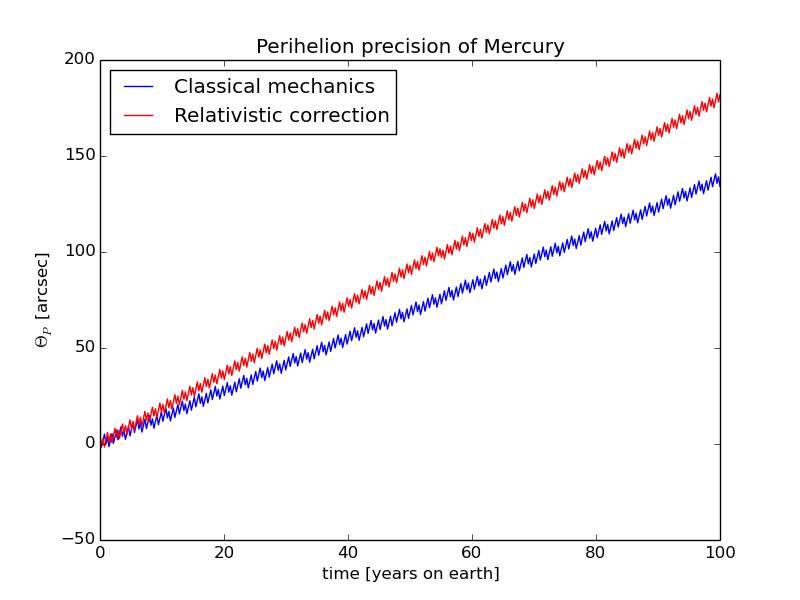
\includegraphics[height=3.2in, width=0.5\textwidth]{perihelion_precision.png} \caption{Perihelion precision for Mercury around the sun for a century. The blue graph represent the classical case and the red graph represent the relativistic case. This is done with $n=10^8$ integrationsteps}
% \end{figure}





% \begin{figure*}[t!]	% a big figure
%     \centering
%     \begin{subfigure}[t]{0.5\textwidth}
%         \centering
%         \includegraphics[height=3.2in]{../omega001.png}
%         \caption{Wavefunction for $\omega_{r} = 0.01$}
%     \end{subfigure}%
%     ~ 
%     \begin{subfigure}[t]{0.5\textwidth}
%         \centering
%         \includegraphics[height=3.2in]{../omega05.png}
%         \caption{Wavefunction for $\omega_{r} = 0.5$}
%     \end{subfigure}

%     \begin{subfigure}[t]{0.5\textwidth}
%         \centering
%         \includegraphics[height=3.2in]{../omega1.png}
%         \caption{Wavefunction for $\omega_{r} = 1$}
%     \end{subfigure}%
%     ~ 
%     \begin{subfigure}[t]{0.5\textwidth}
%         \centering
%         \includegraphics[height=3.2in]{../omega5.png}
%         \caption{Wavefunction for $\omega_{r} = 5$}
%     \end{subfigure}
%     \caption{Two-electron wavefunction for various values of $\omega_{R}$}
% \end{figure*}


\section{Conclusion}
Object orientation makes this mostly easy. Weird flow of the exercices? Implement unit testing?

\section{Appendix}
All code used is available at: %\href{link}{linkname} \\
The programs used in this project are listed in this section:

\begin{description}
\item [main.cpp] Program1
\item [plot.py] Program2
\end{description}

%\tableofcontents 

\end{document}


% \section{\label{sec:level1}First-level heading}

% This sample document demonstrates proper use of REV\TeX~4.1 (and
% \LaTeXe) in mansucripts prepared for submission to APS
% journals. Further information can be found in the REV\TeX~4.1
% documentation included in the distribution or available at
% \url{http://authors.aps.org/revtex4/}.

% When commands are referred to in this example file, they are always
% shown with their required arguments, using normal \TeX{} format. In
% this format, \verb+#1+, \verb+#2+, etc. stand for required
% author-supplied arguments to commands. For example, in
% \verb+\section{#1}+ the \verb+#1+ stands for the title text of the
% author's section heading, and in \verb+\title{#1}+ the \verb+#1+
% stands for the title text of the paper.

% Line breaks in section headings at all levels can be introduced using
% \textbackslash\textbackslash. A blank input line tells \TeX\ that the
% paragraph has ended. Note that top-level section headings are
% automatically uppercased. If a specific letter or word should appear in
% lowercase instead, you must escape it using \verb+\lowercase{#1}+ as
% in the word ``via'' above.

% \subsection{\label{sec:level2}Second-level heading: Formatting}

% This file may be formatted in either the \texttt{preprint} or
% \texttt{reprint} style. \texttt{reprint} format mimics final journal output. 
% Either format may be used for submission purposes. \texttt{letter} sized paper should
% be used when submitting to APS journals.

% \subsubsection{Wide text (A level-3 head)}
% The \texttt{widetext} environment will make the text the width of the
% full page, as on page~\pageref{eq:wideeq}. (Note the use the
% \verb+\pageref{#1}+ command to refer to the page number.) 
% \paragraph{Note (Fourth-level head is run in)}
% The width-changing commands only take effect in two-column formatting. 
% There is no effect if text is in a single column.

% \subsection{\label{sec:citeref}Citations and References}
% A citation in text uses the command \verb+\cite{#1}+ or
% \verb+\onlinecite{#1}+ and refers to an entry in the bibliography. 
% An entry in the bibliography is a reference to another document.

% \subsubsection{Citations}
% Because REV\TeX\ uses the \verb+natbib+ package of Patrick Daly, 
% the entire repertoire of commands in that package are available for your document;
% see the \verb+natbib+ documentation for further details. Please note that
% REV\TeX\ requires version 8.31a or later of \verb+natbib+.

% \paragraph{Syntax}
% The argument of \verb+\cite+ may be a single \emph{key}, 
% or may consist of a comma-separated list of keys.
% The citation \emph{key} may contain 
% letters, numbers, the dash (-) character, or the period (.) character. 
% New with natbib 8.3 is an extension to the syntax that allows for 
% a star (*) form and two optional arguments on the citation key itself.
% The syntax of the \verb+\cite+ command is thus (informally stated)
% \begin{quotation}\flushleft\leftskip1em
% \verb+\cite+ \verb+{+ \emph{key} \verb+}+, or\\
% \verb+\cite+ \verb+{+ \emph{optarg+key} \verb+}+, or\\
% \verb+\cite+ \verb+{+ \emph{optarg+key} \verb+,+ \emph{optarg+key}\ldots \verb+}+,
% \end{quotation}\noindent
% where \emph{optarg+key} signifies 
% \begin{quotation}\flushleft\leftskip1em
% \emph{key}, or\\
% \texttt{*}\emph{key}, or\\
% \texttt{[}\emph{pre}\texttt{]}\emph{key}, or\\
% \texttt{[}\emph{pre}\texttt{]}\texttt{[}\emph{post}\texttt{]}\emph{key}, or even\\
% \texttt{*}\texttt{[}\emph{pre}\texttt{]}\texttt{[}\emph{post}\texttt{]}\emph{key}.
% \end{quotation}\noindent
% where \emph{pre} and \emph{post} is whatever text you wish to place 
% at the beginning and end, respectively, of the bibliographic reference
% (see Ref.~[\onlinecite{witten2001}] and the two under Ref.~[\onlinecite{feyn54}]).
% (Keep in mind that no automatic space or punctuation is applied.)
% It is highly recommended that you put the entire \emph{pre} or \emph{post} portion 
% within its own set of braces, for example: 
% \verb+\cite+ \verb+{+ \texttt{[} \verb+{+\emph{text}\verb+}+\texttt{]}\emph{key}\verb+}+.
% The extra set of braces will keep \LaTeX\ out of trouble if your \emph{text} contains the comma (,) character.

% The star (*) modifier to the \emph{key} signifies that the reference is to be 
% merged with the previous reference into a single bibliographic entry, 
% a common idiom in APS and AIP articles (see below, Ref.~[\onlinecite{epr}]). 
% When references are merged in this way, they are separated by a semicolon instead of 
% the period (full stop) that would otherwise appear.

% \paragraph{Eliding repeated information}
% When a reference is merged, some of its fields may be elided: for example, 
% when the author matches that of the previous reference, it is omitted. 
% If both author and journal match, both are omitted.
% If the journal matches, but the author does not, the journal is replaced by \emph{ibid.},
% as exemplified by Ref.~[\onlinecite{epr}]. 
% These rules embody common editorial practice in APS and AIP journals and will only
% be in effect if the markup features of the APS and AIP Bib\TeX\ styles is employed.

% \paragraph{The options of the cite command itself}
% Please note that optional arguments to the \emph{key} change the reference in the bibliography, 
% not the citation in the body of the document. 
% For the latter, use the optional arguments of the \verb+\cite+ command itself:
% \verb+\cite+ \texttt{*}\allowbreak
% \texttt{[}\emph{pre-cite}\texttt{]}\allowbreak
% \texttt{[}\emph{post-cite}\texttt{]}\allowbreak
% \verb+{+\emph{key-list}\verb+}+.
%
% ****** End of file apssamp.tex ******
